
\chapter{Future Work}
\label{ch: future}


% Rotation and charge flipping
\section[Rotation~UED and Charge Flipping]{Rotation~UED and Charge Flipping}
\label{sec: rotation-CF}

% Intro
Throughout the works in this thesis, UED was demonstrated to be a powerful technique
to elucidate the photoinduced structural dynamics of moderately sized organic molecules
with femtosecond time resolution and atomic spatial resolution.
%
However, there are limits of interpretation to these molecular movies
since the atomic motions were refined using structure models
that are based on crystal structures measured or calculated previously.

% 3D electron diffraction (rotation ED or automated diffraction tomography)
In the field of static electron diffraction, there are now well-demonstrated methods
for solving large complex crystal structures directly~\cite{Mugnaiolia2015}.
%
This is achieved by sampling reciprocal space in all three dimensions
to measure the value of the magnitude of the structure factor $|F(\boldsymbol{q})|$
throughout the spherical volume defined by the spatial resolution
$q_\text{max} \sim 1/\lambda$, where $\lambda$ is the de~Broglie wavelength of the probe electrons,
and applying direct structure refinement algorithms to find
the complex phase $\theta(\boldsymbol{q})$~\cite{Giacovazzo2011, ZouBook}.
%
To make such systematic measurements, there are two experimental techniques:
automated diffraction tomography~(ADT) and rotation electron diffraction~(RED).
%
Briefly, ADT and RED%
\footnote{ADT and RED are electron-diffraction equivalents of the precession and rotation XRD techniques
already in common usage (see Refs.~\cite{Xuong1968, Buerger1964} and~\cite{Arndt1973, ArndtWonacottBook}
respectively).} mechanically tilt the target sample to first roughly sample
reciprocal space; for each sample tilt, ADT precesses the electron beam around the main axis
to integrate the intensity of reciprocal lattice points
that were initially missed~\cite{Kolb2007, Kolb2008, Mugnaiolia2009}
while RED measures a tilt series by finely and incrementally rotating the electron beam
off its axis~\cite{Hovmoller2008, Zhang2010, Wan2013}.

% Rotation UED schematic
\begin{figure}[t!]
  \centering
  \includegraphics[width = \textwidth]{Figures/fig_RotationUED_schematic.pdf}
  \caption[Schematic for rotation UED.]{
    Schematic for rotation UED:
    (a) the overall pump--probe geometry where the sample is rotating around
    (b) the vertical axis (tilting or `yaw') or (c) the longitudinal axis ('roll').
    The right sides of Panels~b and c show the reciprocal-space volume
    that is swept out by these sample rotations.
  }
  \label{fig: Rotation-schematic}
\end{figure}

Here, a variation of UED inspired by ADT and RED --- `rotation UED' ---
is proposed to produce truly ab~initio molecular movies.
%
Fig.~\ref{fig: Rotation-schematic}a shows a schematic of the pump--probe geometry of such an experiment.
%
By inspection, it is not feasible to directly implement the kind of electron-beam steering
and sample rotation necessary for ADT or RED.
%
From Sec.~\ref{sec: UED-setup}, the space between the electron source and the sample
is already occupied by the RF~pulse compression system and cannot be lengthened
to accommodate additional hardware without significantly longer electron pulse durations.
%
Large-angle rotations of the sample would further degrade the temporal resolution setup
by increasing the size of the interaction volume in which there is velocity mismatch
between the electron and laser pulses~\cite{Williamson1993, Siwick2002}.
%
In addition, there would also be ill-constrained variations in the excitation fraction~$\eta_\text{exc}$
of the sample as the direction of the pump laser beam remains fixed
and its incident angle changes over the course of a sample rotation scan.
%
Two solutions to these problems are illustrated in Fig.~\ref{fig: Rotation-schematic}b and c.
%
In Panel~b, tilting of the sample by some small angle~$\phi$ could be pursued
such that a double-wedge shaped volume of reciprocal space is probed with minimal issues.
%
Alternatively, as shown in Panel~c, the sample is tilted off the electron-beam axis
by some angle $\theta \in \left[0, \frac{\unslant[-.2]\pi}{2} \right]$
to align its normal with the laser-beam axis;
at each time point, a spherical region (minus two conical wedges) can be swept out
by a full in-plane rotation.
%
This last geometry for rotation UED is most optimal and was conceived by Dr.~Ryan L. Field.
Indeed, it is a generalization of the Arndt-Wonacott design%
\footnote{Freyer et~al have reported femtosecond XRD results using the Arndt-Wonacott geometry
in reflection mode~\cite{Freyer2011}.} for static rotation XRD~\cite{Arndt1973, ArndtWonacottBook}.

% Euler angle convention: phi, theta, psi
% phi: rotate x around z to align x with N
% theta: rotate z around x'/N
% psi: rotate x' around z'
% (Laudan  Liftschitz, Mechanics, p. 111.)

% Rotation UED data and charge flipping
\begin{figure}[t!]
  \centering
  \includegraphics[width = \textwidth]{Figures/fig_RotationUED.pdf}
  \caption[Making molecular movies with rotation UED and charge flipping.]{
    Making molecular movies with rotation UED and charge flipping:
    rotation UED data of single-crystal silicon in
    (a) camera/sample-tilt coordinates and (b) Cartesian reciprocal coordinates;
    (c) LT~crystal structure of (EDO-TTF)$_2$PF$_6$
    resolved from rotation~UED data using the charge flipping algorithm.
    The inset in Panel~a shows the shape of one relrod
    and the mesh in Panel~c is an isosurface of the reconstructed electrostatic potential.
  }
  \label{fig: Rotation-data}
\end{figure}


% Describe silicon rotation data
Rotation UED by sample tilting was performed in an experiment with single-crystal silicon
and the results are shown in Fig.~\ref{fig: Rotation-data}a and b.
%
Over a $\phi$ scan of $\pm 30^\circ$, all the relrods within the sampled volume could be resolved
as diffraction spots in each image of the rotation series.
In Panel~a, the shape of the electron Ewald sphere can even be discerned by the curvature
in the rows of relrods; in the inset, one exemplary relrod is shown and
it appears to be a composite of a ellipsoid and a sharp spike,
indicating the presence of at least two broadening effects that are at work therein
and which could be analyzed by Zernike- or spectrum-based shape descriptors.
%
In Panel~b, the same dataset is plotted after a coordinate transformation
from the camera/sample-tilt space to Cartesian reciprocal space~\cite{Shaw1981},
which enables easy indexing of all the sampled reciprocal lattice points.

% Charge flipping
There exists many ways%
\footnote{See Ref.~\cite{Palatinus2013b} and the references therein.}
to solve for the real-space crystal structure that underlie the measured reciprocal-space diffraction data;
one of which is the model-based approach that is described in Sec.~\ref{sec: UED-data-analysis-3}
and used throughout the UED works in this thesis.
%
A particularly interesting and powerful method is known as `charge flipping'~(CF)
and it was developed by Oszl\'{a}nyi and S\"{u}t\H{o}~\cite{Oszlanyi2004, Oszlanyi2005,
Oszlanyi2006, Oszlanyi2008, Oszlanyi2011}.
%
First proposed as `low-density elimination'~\cite{Shiono1992, Refaat1993},
CF is an iterative dual-space method for retrieving the missing phase information in crystallography
or finding $\rho(\boldsymbol{r}) \in \mathbb{C}$ given only $|F_\text{exp}(\boldsymbol{q})|$.
%
As described in Ref.~\cite{Palatinus2013b}, this is achieved as follows:
%
\begin{enumerate}
  \item $\rho(\boldsymbol{r}) \xleftarrow[]{\mathcal{F}^{-1}} |F_\text{exp}(\boldsymbol{q})|
    \mathrm{e}^{\mathrm{i} \theta(\boldsymbol{q})}$;
  \item $\rho(\boldsymbol{r}) = \{ \rho(\boldsymbol{r}) \text{ if } \rho(\boldsymbol{r}) \geq \delta,
    -\rho(\boldsymbol{r}) \text{ otherwise} \}$;
  \item $\rho(\boldsymbol{r}) \xrightarrow[]{\mathcal{F}} F(\boldsymbol{q})$;
  \item $F(\boldsymbol{q}) = \{\frac{|F_\text{exp}(\boldsymbol{q})|}{|F(\boldsymbol{q})|} F(\boldsymbol{q})
    \enskip \forall \enskip \boldsymbol{q} \in Q_\text{exp}, F(\boldsymbol{q}) \text{ otherwise} \}$;
  \item $\rho(\boldsymbol{r})\xleftarrow[]{\mathcal{F}^{-1}} F(\boldsymbol{q})$;
  \item go to step 2 until convergence;
\end{enumerate}
%
where $\theta_0(\boldsymbol{q})$ is the initial set of phases which can be choosen at random,
$Q$ is the set of reciprocal lattice points within the experimentally sampled region.
%
Indeed, implicitly assumed here is that a physical $\rho(\boldsymbol{r})$ is (1) sparse%
\footnote{$\rho(\boldsymbol{r})$ can be assumed to be sparse
since it represents quantities --- e.g.~electron density or electrostatic potential ---
that are highly localized at the atomic positions of the crystal structure.}
and (2) strictly positive; no other prior knowledge is necessary~\cite{Eggeman2009}.
%
Thus, applying this algorithm to rotation UED data would enable
a mapping of ultrafast photoinduced molecular motions
without concerns of biases introduced by structure models.

% EDO rotation
A preliminary experiment on single-crystal (EDO-TTF)$_2$PF$_6$ at low temperature
was performed to demonstrate the practical feasibility of rotation UED and charge flipping
on a moderately complex crystal that was previously studied by traditional UED (see Ch.~\ref{ch: UED-EDO}).
%
Rotating by ca. $\pm 45^\circ$, diffraction data of sufficient quality was collected
and piped to the charge-flipping program \texttt{SUPERFLIP}~\cite{Palatinus2007}.
%
Fig.~\ref{fig: Rotation-data}c shows an isosurface of the electronstatic potential that
was found after convergence and the resolved $\text{LT}$ crystal structure of (EDO-TTF)$_2$PF$_6$
as interpreted using the program \texttt{EDMA}~\cite{Palatinus2012}.
%
By inspection, these results are consistent with those reconstructed from static XRD measurements
using traditional means, suggesting that CF is applicable to rotation UED data.

% Future work
% Dynamical effects, multiple scattering reduced~\cite{Mugnaiolia2015}
In the future, a full 4D dataset can be collected using rotation UED
and mapped into an ab~initio molecular movie using charge flipping
to follow the structural dynamics of photoinduced reactions,
including the formation of short-lived intermediate states.
%
In particular, several works (see Ref.~\cite{Mugnaiolia2015} and references therein)
showed that rotation minimizes the effects of dynamical scattering.
%
Developments by Palatinus~et~al~\cite{Palatinus2013a, Palatinus2015a, Palatinus2015b}
offer further means by which to reduce this often-criticized ambiguity of electron diffraction
relative to XRD, improving the spatial resolution to a point
where hydrogen atoms could even be resolved~\cite{Palatinus2017}.


% SVD of UED image stack
\section[Dimensionality Reduction of UED Image Stack]{Dimensionality Reduction of UED Image Stack}
\label{sec: UED-SVD}

In the UED works of this thesis, data analysis was carried out
on the bundle of individual time traces that were integrated
over the area of each observable reciprocal lattice point.
%
From Sec.~\ref{sec: UED-data-analysis-2},
the dimensionality of the dataset, as determined by the size of this bundle,
can be drastically reduced by singular value decomposition~(SVD).
%
Not described was the possibility of applying SVD directly on the UED image stack
itself.
%
This approach was not feasible given that it involved storing and computing
matrices of size $M \times M$, where $M \sim 2000$ is the pixel dimension of a UED image.
%
However, a trick was conceived recently to avoid this memory bottleneck
and it is described preliminarily as follows.


A UED dataset is composed a sequence of images captured by the CCD~camera
measuring the diffraction pattern of the sample as a function of time delay~(see Fig.~\ref{fig: UED-SVD}a).
This forms a 3D image stack of size $M \times M \times N$,
where $M$ and $N$ are respectively the pixel dimension of each image and the number of sampled time points.
%
Indexing the pixels linearly, a familiar but very large 2D matrix is obtained,
%
\begin{equation}
  \begin{aligned}
    \Delta I(t, \boldsymbol{q}) \rightarrow \mathbf{\Delta I} =
    \begin{bmatrix}
        \Delta I(t_1, \boldsymbol{q}_1) & \cdots & \Delta I(t_N, \boldsymbol{q}_1) \\
        \vdots & \ddots & \vdots \\
        \Delta I(t_1, \boldsymbol{q}_{M^2}) & \cdots & \Delta I(t_N, \boldsymbol{q}_{M^2})
    \end{bmatrix}
  \end{aligned}
\end{equation}
%
where $\boldsymbol{q}$ spans not just the diffraction spots but all the reciprocal space
that is resolved on the CCD~sensor.
%
Instead of directly solving for $\mathbf{U}, \mathbf{S}, \mathbf{V}$,
it is partitioned along $i = 1 \dots M^2$ into many smaller matrices $\mathbf{\Delta I}_k$,
which can be easily decomposed by QR~factorization,
%
\begin{equation}
  \begin{aligned}
    \mathbf{\Delta I} =
    \begin{bmatrix}
        \mathbf{\Delta I}_1 \\
        \vdots \\
        \mathbf{\Delta I}_K
    \end{bmatrix} \\
    \mathbf{\Delta I}_k = \mathbf{Q}_k \mathbf{R}_k
  \end{aligned}
\end{equation}
%
where $\mathbf{Q}_k, \mathbf{R}_k$ are a pair of orthogonal and triangular matrices.
%
Then, $\mathbf{S}, \mathbf{V}$ can be simply calculated by applying~SVD
on $[ \mathbf{R}_1 \dots \mathbf{R}_K ]^\mathsf{T}$ to the first $N$ rows.
%
The matrix $\mathbf{U}$ is finally obtained
by computing the inverse of the $N \times N$ square matrix $\mathbf{S} \mathbf{V}^\mathsf{T}$
and multiplying it with $\mathbf{\Delta I}$.

% SVD of UED image stack
\begin{figure}[t!]
  \centering
  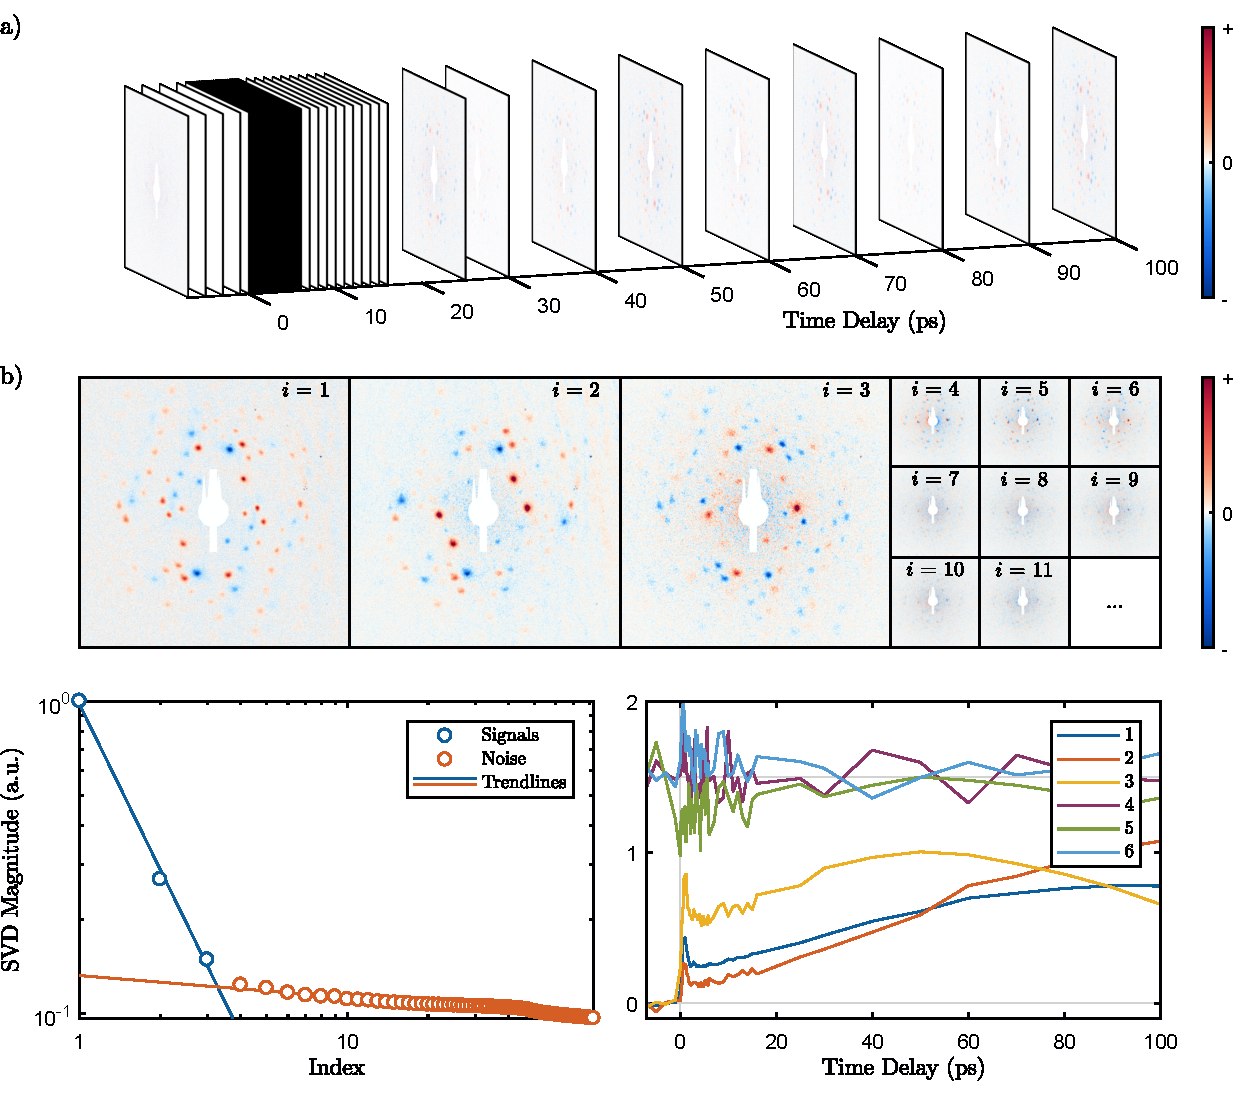
\includegraphics[width = \textwidth]{Figures/fig_UED_imageSVD.pdf}
  \caption[Dimensionality reduction of UED image stack.]{
    Dimensionality reduction of UED image stack:
    (a)~A UED dataset is a sequence of images that can be interpreted
    as a stack in the axis of time delay;
    (b)~singular value decomposition can be applied directly to this 3D array,
    producing its left singular vectors~(top), singular values~(left),
    and right singular vectors~(right), where $i$ is the index.
    The results shown here are those calculated from the (EDO-TTF)$_2$PF$_6$ dataset
    described in Sec.~\ref{sec: UED-EDOPF6}.
  }
  \label{fig: UED-SVD}
\end{figure}

Fig.~\ref{fig: UED-SVD}b shows the results of the above method being applied
on the UED dataset of (EDO-TTF)$_2$PF$_6$.
%
Indeed, three principal components are recovered with dynamics consistent with
those found prior by SVD of the time traces.
%
Additionally, inspection of the left singular vectors in $\mathbf{U}$
reveals that the next strongest components are displacive features,
suggesting that beampointing errors can be neatly separated from
the UED signal without peak fitting.

Note that the above method is distinct from that reported by Schmidt et~al in Ref.~\cite{Schmidt2003},
wherein SVD-based global lifetime analysis can only be applied after successful reconstruction
of the entirety of electron density maps in real space.
Here, the time-resolved data could be interpreted directly in reciprocal space,
bypassing the need to collect and model a full UED dataset.


% Frequency analysis of BPY TA data
\section[Frequency Analysis of \protect{[Fe\textsuperscript{II}(bpy)\textsubscript{3}]\textsuperscript{2+}}
TA Data]{Frequency Analysis of \protect{[Fe\textsuperscript{II}(bpy)\textsubscript{3}]\textsuperscript{2+}} TA Data}
\label{sec: freq-anal-BPY}

In Sec.~\ref{sec: TA-BPY}, the results of a broadband TA measurement of BPY were described.
Figs.~\ref{fig: BPY-data-aqueous-resi} and~\ref{fig: BPY-data-crystal-resi}
showed that a complex pattern of oscillations exists within the GA~fit residuals
of the UV--Vis spectra of both the solvated and single-crystal samples.
%
These features were analyzed by calculating the Fourier transform of the data
using the Welch's method over all time delays and assigning heuristically the peaks therein
to known vibrational modes of the molecule and phonons of the bulk lattice
(see Figs.~\ref{fig: BPY-data-aqueous-Welch} and~\ref{fig: BPY-data-crystal-Welch}).
%
Although simple, this approach to frequency analysis is not ideal
since it lacks time windowing and thus obviates the time-resolved nature of the experimental data.
%
In particular, photophysical processes and atomic motions can give rise to
time-dependent modulations in both the amplitude and frequency of the probe signal.
%
It would be remiss to neglect such transients of interest.

% Wavelet figure
\begin{figure}[ht!]
  \centering
  \includegraphics[width = \textwidth]{Figures/fig_BPY_TA_CWT.pdf}
  \caption[Frequency analysis using continuous wavelet transform.]{
    Frequency analysis using continuous wavelet transform:
    (a) UV short-time TA data of solvated BPY
    and (b) the calculated scalogram
    where the 3D~power spectrum is represented by the isosurface plot of the wavelet magnitude.
    The $xy$, $xz$, and $yz$ panels show the wavelet magnitude
    averaged along the axis of wavelet wavenumber, probe wavelength,
    and time delay;
    the black dashed lines specify values of interest
    while the blue one delimites the cone of influence.
  }
  \label{fig: BPY-TA-CWT}
\end{figure}

Here, it is proposed to apply the continuous wavelet transform~(CWT)
instead of the fast Fourier transform~(FFT) to analyze the measured broadband TA signals
in time, probe wavelength, and frequency simultaneously~\cite{WaveletBook}.
%
This approach is demonstrated in Fig.~\ref{fig: BPY-TA-CWT}
using the GA~residuals of the UV short-time spectra of solvated BPY (Panel~a).
%
To generate the 3D power spectrum in Panel~b, CWT%
\footnote{The continuous wavelet transform is calculated
using the \texttt{cwt} function in \textsc{MATLAB}~R2017b
where the wavelet is chosen to be
the default `Morse' wavelet~\cite{Olhede2002, Olhede2012},
named for American physicist Philip M. Morse (1903--1985) who first derived
it as the solution to the Schr\"{o}dinger wave equation with
his eponymous potential energy function~\cite{Morse1929}.}
is applied to the time scan of each probe wavelength.
%
The transient CPM~signal near $t = 0$~ps produces an intense broadband feature
that obscures the early-time dynamics.
Its contribution is removed by constructing a~$\Delta A_\text{CPM}(t, \lambda)$
and subtracting its power spectrum from the original one as follows:
%
\begin{equation}
  \begin{aligned}
    \Delta A_\text{CPM}(t, \lambda) & =
      \begin{cases}
        \Delta A(t, \lambda), & \text{if } t_\text{min} \leq 0 \\
        \Delta A(-t, \lambda), & \text{if } 0 < t \leq -t_\text{min} \\
        0, & \text{if } -t_\text{min} < t < t_\text{max} \\
      \end{cases}
      \\
    \text{CWT}[\Delta A(t, \lambda)]
      & \rightarrow \text{CWT}[\Delta A(t, \lambda)] - \text{CWT}[\Delta A_\text{CPM}(t, \lambda)]
  \end{aligned}
\end{equation}
%
where $t = [t_\text{min}, t_\text{max}]$.

From the example in Fig.~\ref{fig: BPY-TA-CWT},
the singular oscillation of the FFT~power spectrum at $\nu = 128$~cm$^{-1}$
(see Fig.~\ref{fig: BPY-data-aqueous-Welch}) is recovered
in the CWT~power spectrum as a spectral feature centered at $\lambda = 315$~nm
that appears at $t = +0$~ps and evolves from ca.~$160$~cm$^{-1}$ to ca.~$120$~cm$^{-1}$.
%
These wavenumber values remain consistent with the earlier assignment
to a Fe--N stretching mode of the LS molecule that has been activated by
impulsively stimulated Raman scattering.
%
However, two alternative assignments are also possible
if the shape of this feature over time is interpreted as either
a single mode downshifting in frequency or one mode converting into a lower one.
%
Assuming that there is substantial ESA contribution to this GSA-dominated spectral region,
the former could represent vibrational wavepacket motion
on a HS potential energy surface that is softening along the Fe--N reaction coordinate
as the excited state relaxes via~IVR~\cite{Aubock2015};
the latter may be a proxy for the population transfer from the LS or MLCT~states
to the HS~state~\cite{Cammarata2014, Bertoni2015}.


% UED BPY work
\section[Structural Dynamics of Spin Crossover in \protect{[Fe\textsuperscript{II}(bpy)\textsubscript{3}](PF\textsubscript{6})\textsubscript{2}}]{Structural Dynamics of Spin Crossover in \\ \protect{[Fe\textsuperscript{II}(bpy)\textsubscript{3}](PF\textsubscript{6})\textsubscript{2}}}
\label{sec: UED-BPY}

% UED patterns and time traces
\begin{figure}[b!]
  \centering
  \includegraphics[width = \textwidth]{Figures/fig_BPY_UEDimages.pdf}
  \caption[UED data of single-crystal BPY.]{
    UED data of single-crystal BPY:
    (a) static image of the LS phase at room temperature;
    difference image between the pump-on and pump-off states
    at (b) $t = +4$~ps and (c) $t = +100$~ps;
    (d) difference image simulated using the crystal structure model
    set to $\boldsymbol{\xi} = (1, 1, 1, 1)$ and $\boldsymbol{\xi} = (0, 0, 0, 0)$;
    (e) time traces of select diffraction spots showcasing
    the biexponential nature of the underlying structural dynamics.
  }
  \label{fig: BPY-UEDimages}
\end{figure}

% Introduction
The ultrafast dynamics of photoinduced SCO was studied twofold in this thesis:
electronically using femtosecond UV--Vis TA spectroscopy in solution and single-crystal~BPY
(Sec.~\ref{sec: TA-BPY}); structurally using UED in single-crystal~AZA (Sec.~\ref{sec: UED-AZA}).
%
While there are previous reports on both the electronic dynamics of AZA~\cite{Marino2013, Marino2016}
and the structural dynamics of BPY~\cite{Gawelda2007b, Bressler2009, Haldrup2012, Freyer2013,
Haldrup2016, Lemke2017, Kjaer2017a}, unanswered questions remain.
%
For one, neither time-resolved broadband absorption spectra
nor a linear absorption spectrum has been taken of AZA,
probably as a result of its high absorptivity and
the general unavailability of optically thin samples.
%
Similarly, no one has performed a direct and low-excitation measurement
of the entire molecular structure of BPY while it undergoes radiationless transitions
and relaxes from the MLCT manifold back down to the HS state.
%
As such, there are obvious blind spots in the literature picture
of the structure--function correlation in light-induced SCO on the ultrafast time scale
(see Sec.~\ref{sec: SCO-photo-4}).
%
Here, I present some preliminary UED results on single-crystal BPY
that were obtained recently and are part of a manuscript in preparation for publication.

% Methods
The UED experiment on single-crystal BPY was performed in a manner
that is analogous to that done on AZA in Sec.~\ref{sec: UED-AZA}
but using a 400-nm pump pulse for photoexcitation.
%
The peak pump fluence was set to ca. 5.12~mJ/cm$^2$ (85~GW/cm$^2$)
to excite the 150-nm ultrathin sample within the single-photon linear regime,
as in the case of Ref.~\cite{Aubock2015} and Sec.~\ref{sec: TA-BPY}.
The pump--probe repetition rate was also set to $50$~Hz to allow for
full $\text{LS} \leftarrow \text{HS}$ relaxation and dissipation of laser-deposited heat.
%
Based on the literature XRD~\cite{Dick1998} and TA~\cite{Zhang2014, Field2016} data,
the excitation fraction here was calculated to be ca. 34~\%.

% Results
Fig.~\ref{fig: BPY-UEDimages}a shows the static UED image taken
of the BPY sample at room temperature.
A large number of diffraction spots are readily visible,
suggesting high crystallinity.
Using the published XRD crystal structure and the refinement procedure
described in Sec.~\ref{sec: UED-data-analysis-3},
the crystal orientation of the sample was determined to be $[2 1 0]$.

% Molecular movie
\begin{figure}[t!]
  \centering
  \includegraphics[width = \textwidth]{Figures/fig_BPY_UED_Xi.pdf}
  \caption[Molecular movie of single-crystal BPY.]{
    Molecular movie of single-crystal BPY as reconstructed
    from its UED data using (a) the crystal structure model of four dynamical groups:
    (b) Fe--N bond elongation (red), Fe--ligand elongation (yellow),
    Fe--N rotation (green), Fe--ligand rotation (blue).
  }
  \label{fig: BPY-UED-Xi}
\end{figure}

Time-resolved pump--probe results are shown in the images of Figs.~\ref{fig: BPY-UEDimages}b
and c, where $t = +4$~ps and $t = +100$~ps respectively,
and in the time traces of Fig.~\ref{fig: BPY-UEDimages}d.
%
These measured difference images can be directly compared with
that in Panel~d, which is simulated using the crystal structure of the LS
and HS states. While the former is known from literature~\cite{Dick1998},
the latter is generated from a 4D~BPY structure model (see Fig.~\ref{fig: BPY-UED-Xi}a)
based on the computational work of Daku and Hauser~\cite{Daku2010}:
%
\begin{enumerate}
  \item Fe--N bond elongation;
  \item Fe--ligand elongation;
  \item Fe--N rotation;
  \item Fe--ligand rotation.
\end{enumerate}

Given the close match between the $+4$-ps pattern and the simulated one,
the plateau that forms on the few-picosecond time scale can be assigned
to the photoexcited HS state.

% Diagram of reaction pathways
\begin{figure}[b!]
  \centering
  \includegraphics[width = \textwidth]{Figures/fig_BPY_UED_picture.pdf}
  \caption[Schematic of the proposed SCO reaction pathways of BPY and AZA.]{
    Schematic of the proposed SCO reaction pathways of (a) BPY and (b) AZA
    within their respective configuration space, as evidenced by the UED data.
    The left panels show the principal right singular vector of BPY and AZA,
    fitted to highlight the biexponential and monoexponential nature of their dynamics.
  }
  \label{fig: BPY-UED-picture}
\end{figure}

As before, a molecular movie of BPY can be reconstructed from the measured UED data
by optimizing the structure model $\boldsymbol{\xi} = (\xi_1, \xi_2, \xi_3, \xi_4)$
against the relative intensity changes of all the visible diffraction spots.
%
The resulting values and fits are shown in Fig.~\ref{fig: BPY-UED-Xi}b.
%
By inspection, the photoinduced SCO process converts the crystal structure of BPY
from the LS state $\boldsymbol{\xi} = (0, 0, 0, 0)$ to a HS-like one
at $\boldsymbol{\xi} = (0.98, 0.84, 0.95, 0.83)$
by driving the Fe--N modes more strongly than the Fe--ligand modes.
%
In real space, these reaction coordinates translates into
a Fe--N bond elongation and rotation of ca.~$0.15$~\AA{} and $2.2^\circ$
and Fe--ligand motion of ca.~$0.17$~\AA{} and $2.5^\circ$.

% Time constants and pathways
Global analysis of the entire UED data set reveals that
the structural dynamics of single-crystal BPY is biexponential in nature,
with two time constants: $\tau_1 = (445 \pm 230)$~fs and $\tau_2 = (2.43 \pm 0.37)$~ps.
%
From earlier optical and X-ray spectroscopic studies in the related compound
$\mathrm{[Fe^{II}(phen)_2(NCS)_2]}$~\cite{Cammarata2014, Bertoni2015},
the fast step can be interpreted as a rapid and correlated expansion of the $\mathrm{FeN_6}$ core
driven by the radiationless transition from the MLCT manifold
onto the steep potential energy surface of the HS state.
%
Given the values of $\tau_2$ and $\boldsymbol{\xi}(t)$,
the slow step is consistent with atomic motions associated with IVR,
wherein the BPY molecule reorganizes and ligand modes are activated
to dissipate the large amount of excess energy.
%
In Fig.~\ref{fig: BPY-UED-picture}, this two-step behaviour of BPY
is contrasted with the one-step one that was described for single-crystal AZA
in Sec.~\ref{sec: UED-AZA} and the TR-XRD results of Freyer~et~al
measured in powder~BPY~\cite{Freyer2013}.
%
At this time, it is hypothesized that the disparate structural dynamics
reflects the greater size and lower symmetry of AZA relative to BPY
and how these structural differences affect the ultrafast function of SCO.

\section{Application of Deep Learning to UED}
\label{sec: future-deep}

% Problem
In Secs.~\ref{sec: TA-data-analysis} and~\ref{sec: UED-data-analysis-2},
I described extensively the many methods that I developed and applied for analyzing TA and UED data.
%
A common refrain therein is the voluminous amount of work needed
in both the lab for gathering sufficient measurements for statistical significance
and on the desktop for curating and denoising data.
%
One reason for this issue is the SNR limitation inherent to the pump--probe experimental scheme.
In femtosecond TA spectroscopy, neither the pump nor the probe can be too bright
since both the sample and the detector of the spectrometer can be saturated or damaged.
This holds true for UED as well, with the additional problem of
a show-stopping loss of subpicosecond temporal resolution
due to the Coulomb explosion of overly packed electron bunches.

% Denoising by deep learning (convolutional neural network)
An impressive accessory to the present scheme for the preprocessing of UED~image data
would be denoising of TA spectra and UED images by an obvious application
of `deep learning' methods~\cite{LeCun2015}.
%
As proposed for fluorescence microscopy in Ref.~\cite{Weigert2018},
low- and high-SNR measurements would be made either with variable laser fluence
to pump a stand-in sample with a high threshold for photodamage or
variable probe brightness on the sample of interest in the steady/dark state.
%
These images would constitute the input--output pairs used to train and validate
an ensemble of convolution neural networks:
the weights become optimized by backpropagation to `restore' the low-SNR images
to the high-SNR counterparts.
%
Thus, an experimental unattainable high-SNR TA or UED dataset could be achieved
as predictions from these networks when given low-SNR measurements as input
and the variance within the ensemble would be defined as the prediction error.


% Other molecular systems
\section[Other Molecular Systems of Interest]{Other Molecular Systems of Interest}
\label{sec: future-molecules}

In this thesis, three topical types of photoactive molecular crystals were investigated by UED:
the insulator--metal phase transition in Bechgaard-Fabre salts (Ch.~\ref{ch: UED-EDO}),
photocyclization of a diarylethene (Ch.~\ref{ch: UED-DAE}), and
spin~crossover in transition metal complexes (Ch.~\ref{ch: SCO}).
%
Future experiments may study similar but composite molecular systems as toy models
for validate the lessons in molecular design learnt from the prior works
and explore the interaction between the physics and chemistry innate to
each of the components.
Of particular interest are those shown in Fig.~\ref{fig: future-molecules}
that were identified in literature%
\footnote{See Refs.~\cite{Brachnakova2018, Chastanet2018} and the references therein.}
to have the spin state of their metal centre becoming coupled to the conformational state
of the ligands and/or the counterions.

% Diagram of reaction pathways
\begin{figure}[ht!]
  \centering
  \includegraphics[width = \textwidth]{Figures/fig_future_mol.pdf}
  \caption[Other molecular systems of interest for future UED work.]{
    Other molecular systems of interest for future UED work:
    (a)~[Fe$^\text{II}$(H$_2$B(pz)$_2$)$_2$(phen*)]~\cite{Milek2013};
    (b)~[Ni$^\text{II}$(TPP)(PAP)]~\cite{Venkataramani2011};
    (c)~[Fe$^\text{II}$(dpp-TTF)$_2$] [Ni$^\text{II}$(mnt)$_2$]$_2$(BF$_4$)~\cite{Nihei2011}.
  }
  \label{fig: future-molecules}
\end{figure}

% Abbreviations:
% [H$_2$B(pz)$_2$]$^-$: bis(hydrido)-bis(1\textit{H}-pyrazolyl)borate,
% L = 5,6-bis(2,5-methyl-3-thienyl)-1,10-phenanthroline,
% TPP$^{2-}$ = tris(pentafluorophenyl)porphyrin,
% PAP = 3-(phenylazo)pyridine,
% dpp = 2-{2,6-bis(1-pyrazolyl)pyridyl}-ethylene,
% TTF = tetrathiafulvalene,
% mnt$^-$ = maleonitriledithiolate.

% SCO + others?
% Ligand-driven light-induced spin transition in spin crossover compounds
% Brachnakova and Salitros, 2018

% X[M(dmit)2]2, M(dmit) is isolobal to BEDT-TTF
% Review in 1991: Molecular metals and superconductors derived
% from metal complexes of 1,3-dithiole-2-thione-4,5-dithiolate (dmit)
% (the abbreviation dmit originates from the obsolete name for dimercaptoisotrithione)








%
